%%%%%%%%%%%%%%%%%%%%%%%%%%%%%%%%%%%%%%%%%%%%%%%%%%%%%%%%
\fondo{celeste}
\section{¿Cómo funciona ChatGPT?}
\fondo{blanco}
%%%%%%%%%%%%%%%%%%%%%%%%%%%%%%%%%%%%%%%%%%%%%%%%%%%%%%%%


%%%%%%%%%%%%%%%%%%%%%%%%%%%%%%%%%%%%%%%%%%%%%%%%%%%%%%%%
\begin{frame}{¿Cuál es la próxima palabra?}

\begin{center}
\begin{tikzpicture}[>=Stealth, font=\sffamily]

% Nodo principal
\node[draw, rounded corners, fill=white, minimum height=1cm, text width=3.5cm, align=center] (contexto) {El niño fue al};

% Coordenadas de destinos
\coordinate (out) at ($(contexto.east)+(1.5,0)$);

\coordinate (cafe)     at ($(out)+(1, 2.1)$);
\coordinate (hospital) at ($(out)+(1, 1.05)$);
\coordinate (parque)   at ($(out)+(1, 0)$);
\coordinate (escuela)  at ($(out)+(1, -1.05)$);
\coordinate (banco)    at ($(out)+(1, -2.1)$);

% Textos
\node[anchor=west, text=green!60!black]  at (cafe)     {\textbf{\textcolor{green!70!black}{Café}}};
\node[anchor=west, text=blue!80!black]   at (hospital) {\textbf{\textcolor{blue!80!black}{Hospital}}};
\node[anchor=west, text=violet]          at (parque)   {\textbf{\textcolor{violet}{Parque}}};
\node[anchor=west, text=red]             at (escuela)  {\textbf{\textcolor{red}{Escuela}}};
\node[anchor=west, text=brown!70!black]  at (banco)    {\textbf{\textcolor{brown!70!black}{Banco}}};

% Flechas en forma de L
\draw[->] (contexto.east) -- ++(1.5,0) |- (cafe);
\draw[->] (contexto.east) -- ++(1.5,0) |- (hospital);
\draw[->] (contexto.east) -- ++(1.5,0) |- (parque);
\draw[->] (contexto.east) -- ++(1.5,0) |- (escuela);
\draw[->] (contexto.east) -- ++(1.5,0) |- (banco);

\end{tikzpicture}
\end{center}
\end{frame}
%%%%%%%%%%%%%%%%%%%%%%%%%%%%%%%%%%%%%%%%%%%%%%%%%%%%%%%%

%%%%%%%%%%%%%%%%%%%%%%%%%%%%%%%%%%%%%%%%%%%%%%%%%%%%%%%%
\begin{frame}{¿Cuál es la próxima palabra?}

\begin{center}
    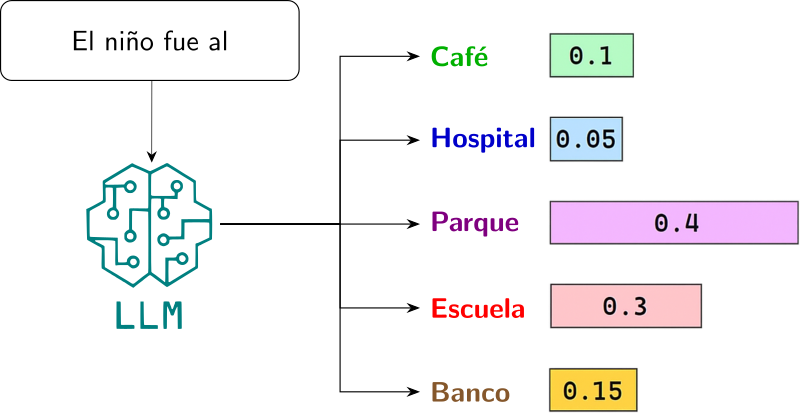
\includegraphics[width=0.8\linewidth]{Figuras/Fig03.png} 
\end{center}
\end{frame}
%%%%%%%%%%%%%%%%%%%%%%%%%%%%%%%%%%%%%%%%%%%%%%%%%%%%%%%%



%%%%%%%%%%%%%%%%%%%%%%%%%%%%%%%%%%%%%%%%%%%%%%%%%%%%%%%%
\begin{frame}{¿Cómo funciona ChatGPT?}
\begin{columns}
\column{0.7\textwidth}
\begin{block}{}
\begin{itemize}
    \item ChatGPT es una herramienta que usa los Modelos GPT de OpenAI.
    \item Los modelos GPT de OpenAI son \textbf{ modelos grandes de lenguaje} (\textit{Large Language Model}, LLM).
    \item Su tarea principal es predecir la \textbf{palabra más probable} dada una secuencia anterior.
    \item No comprende el significado, solo calcula probabilidades a partir de patrones lingüísticos aprendidos.
\end{itemize}
\end{block}
\column{0.3\textwidth}

\includegraphics[width=0.9\linewidth]{Figuras/Fig04.png} 
\end{columns}
\end{frame}
%%%%%%%%%%%%%%%%%%%%%%%%%%%%%%%%%%%%%%%%%%%%%%%%%%%%%%%%


%%%%%%%%%%%%%%%%%%%%%%%%%%%%%%%%%%%%%%%%%%%%%%%%%%%%%%%%
\begin{frame}[t]{Predicción de la siguiente palabra}
\begin{columns}
\column{0.3\textwidth}
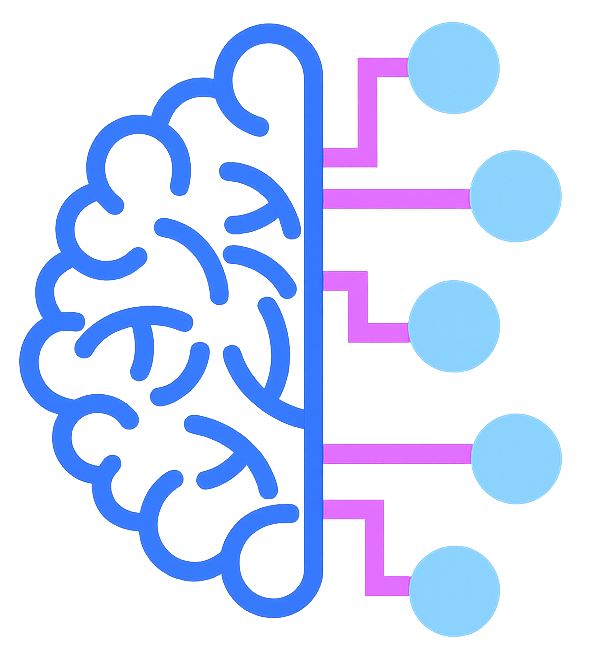
\includegraphics[width=0.9\linewidth]{Figuras/Fig05.png} 
\column{0.7\textwidth}
\begin{block}{}
\begin{itemize}
    \item El modelo asigna una \textbf{distribución de probabilidades} a cada posible palabra siguiente.
    \item No elige al azar: selecciona las opciones con mayor probabilidad.
    \item Por eso puede generar respuestas coherentes... o también \textbf{erróneas} de manera convincente.
\end{itemize}
\end{block}
\end{columns}
\end{frame}
%%%%%%%%%%%%%%%%%%%%%%%%%%%%%%%%%%%%%%%%%%%%%%%%%%%%%%%%


\begin{frame}[t]{¿Cómo se entrenó ChatGPT?}
\begin{itemize}
    \item GPT-3 fue entrenado con más de \textbf{300 mil millones de tokens} ($\sim $570 GB de texto limpio).
    \item Para GPT-4 se utilizó un volumen mucho mayor, aunque OpenAI no ha revelado cifras exactas.
\end{itemize}

\vspace{0.3cm}
\begin{block}{Fuentes principales}
\begin{itemize}
    \item \textbf{Common Crawl} (filtrado y depurado).
    \item \textbf{WebText2}, \textbf{Books1}, \textbf{Books2}, y \textbf{Wikipedia en inglés}.
\end{itemize}
\end{block}
\end{frame}